% =====================================================================
% The Economics of Inward Migration
% Tim Swanson — The Omega Centauri Society / Post Oak Labs
% Paper D of five. Target: omegacentauri.me -> arXiv.
% Build: pdflatex economics-paper && bibtex economics-paper && pdflatex x2
% Bibliography: references.bib + campaign-extra.bib + inward-extra.bib
%               + economics-extra.bib
% =====================================================================
\documentclass[11pt]{article}

\usepackage[margin=1.1in]{geometry}
\usepackage{newtxtext,newtxmath}
\usepackage[round,authoryear]{natbib}
\usepackage{graphicx}
\usepackage{booktabs}
\usepackage{amsmath} % amssymb omitted: newtxmath already provides AMS symbols
\usepackage{tikz}
\usepackage{pgfplots}
\pgfplotsset{compat=1.17}
\usetikzlibrary{arrows.meta,positioning,shapes.geometric}
\usepackage[font=small,labelfont=bf]{caption}
\usepackage{microtype}
\usepackage[colorlinks=true,linkcolor=blue!50!black,citecolor=blue!50!black,urlcolor=blue!50!black]{hyperref}
\usepackage{xcolor}

\newcommand{\msun}{\ensuremath{M_\odot}}
\newcommand{\astar}{\ensuremath{a_\star}}
\newcommand{\kb}{\ensuremath{k_{\mathrm{B}}}}
\newcommand{\specbox}[1]{\par\smallskip\noindent\fbox{\parbox{0.97\linewidth}{\small\textbf{Epistemic status:} #1}}\smallskip\par}

\title{\textbf{The Economics of Inward Migration:\\ Relocation versus Densification for Computation-Maximizing Civilizations}}
\author{Tim Swanson\\[2pt]
\small The Omega Centauri Society / Post Oak Labs\\
\small \texttt{tim@postoaklabs.com}}
\date{July 2026 \\[4pt] \small Draft v1.4 (last revised 2026-07-30) --- fourth paper of the set; companion to \emph{The Macro Transcension Hypothesis} (Paper A), the inward-migration review (Paper B),\\ \small the Omega Centauri campaign (Paper C), and the engineered-IMBH systems paper (Paper E);\\ \small prepared for omegacentauri.me}

\begin{document}
\maketitle

\begin{abstract}
\noindent
The inward-migration resolutions of the Fermi paradox hold that computation-optimizing civilizations relocate to thermodynamically privileged environments, with rapidly spinning intermediate-mass black holes (IMBHs) in dense old clusters as the strongest candidate destination. \citet{Bostrom2003} priced the opportunity cost of delayed expansion and \citet{Bennett2019} priced the losses of dormancy, but relocation itself, the abandonment of accumulated local infrastructure for a transit of $10^{4}$--$10^{6}$ years toward a large deferred payoff, has never been priced. This paper treats that trade as a decision problem over a common utility (discounted integrated computation) with three strategies: stay-and-densify (Matrioshka-style local engineering), migrate (beamed-sail relocation to the nearest suitable IMBH cluster), and seed-and-stay (a self-replicating seed dispatched while densification continues at home). Using payoff kernels assembled from established physics, we derive closed-form crossover conditions.

\medskip
\noindent
The central result is a threshold on the effective discount-plus-hazard rate: migration dominates densification whenever $\rho + \lambda < \ln(G p_{s})/\tau$, where $G$ is the destination computation-rate multiplier ($10^{6}$--$10^{9}$ on power alone, depending on fuel imports), $p_{s}$ the transit survival probability, and $\tau$ the transit-plus-construction time. At fiducial parameters the threshold is $\rho + \lambda \lesssim 2\times10^{-4}$~yr$^{-1}$: any lineage whose combined discount-plus-hazard half-life exceeds roughly $3{,}500$ years should migrate. The seed-and-stay hybrid dominates both pure strategies throughout the migration-favourable region and in a band extending modestly beyond the threshold (to $\rho+\lambda \approx 1.7\,\rho^{*}$ at a physical seed cost $f = 10^{-6}$), because seed mass is a negligible fraction of local output; beyond that band the exponential discount on the deferred payoff extinguishes the seed's value. Embedding the decision rule in a mixed population quantifies how much inward migration thins the expected loud population, and yields a new population-level residue: the predicted sky ratio of Matrioshka-type infrared sources to quiet-cluster systems, which archival infrared nulls constrain once residue lifetimes are folded in. All results are conditional on the optimization premise shared by the hypothesis family; the contribution is the pricing structure, not the premise.
\end{abstract}

\bigskip
\noindent\textbf{Keywords:} Fermi paradox; SETI; technosignatures; transcension; migration; decision theory; discounting; intermediate-mass black holes; Dyson spheres

\newpage
\tableofcontents
\newpage

% =====================================================================
\section{Introduction}
\label{sec:intro}

\subsection{The pricing gap}

Three papers precede this one. The Macro Transcension Hypothesis \citep[hereafter Paper A]{Swanson2026MTH} argues that rapidly spinning massive black holes in dense old stellar systems are the global optimum among present-day environments for long-term computation, and identifies Omega Centauri as the most accessible test system. A critical review of the inward-migration family \citep[hereafter Paper B]{Swanson2026Review} places that hypothesis among six decades of related proposals and grades their falsifiability. An observational companion \citep[hereafter Paper C]{Swanson2026Campaign} specifies the instrument-matched campaign. Paper B also catalogued the family's open problems, and its third problem motivates this paper directly: the economics of the migration itself has never been worked out.

The gap is specific. \citet{Bostrom2003} priced delay: every century of postponed expansion forgoes an irrecoverable harvest of free energy. \citet{Bennett2019} priced dormancy: free energy not collected promptly is lost, so the aestivation strategy of \citet{Sandberg2016} forfeits most of what it hoped to save. Nobody has priced relocation. A lineage that migrates abandons its accumulated local infrastructure, spends $10^{4}$--$10^{6}$ years in transit, accepts a risk of total loss en route, and only then begins to collect a payoff that is, by the physics of Paper A, orders of magnitude larger per unit of everything. Whether that trade clears depends on quantities the inward-family literature has so far left unmodelled: discount rates, hazard rates, transit risk, and the option of sending a seed instead of moving.

This matters beyond bookkeeping. If migration clears the trade only for implausibly patient agents, the inward family loses its force as a Fermi solution regardless of the destination physics. If it clears easily, the family's incomplete-compliance problem (Paper B, problem P4) sharpens into a quantitative question: what fraction of lineages must migrate for the observed silence to follow? Either outcome constrains the family.

\subsection{Claims and non-claims}
\label{sec:claims}

\specbox{This paper is decision theory over established physics. It makes no claim that extraterrestrial intelligence exists. Every result is conditional on the optimization premise (P1 of Paper A): that some long-lived technological lineages maximize long-term computation. The contribution is the pricing structure and its observational corollaries.}

The paper makes three claims:

\begin{enumerate}
\item \textbf{(Decision analysis.)} Under the stated utility and payoff kernels, the choice among stay, migrate, and seed-and-stay reduces to closed-form threshold conditions on the discount rate, hazard rate, transit time, and destination multiplier (Section~\ref{sec:crossover}).
\item \textbf{(Hybrid boundary.)} Under additive utility and the seed-fidelity assumption made explicit in Section~\ref{sec:hybrid}, the seed-and-stay hybrid weakly dominates both pure strategies wherever migration clears, a near-immediate consequence of a nearly free seed; the substantive result is the narrowness of the band beyond the threshold in which the hybrid still pays, $\rho+\lambda \approx 1.7\,\rho^{*}$ at seed cost $f = 10^{-6}$, because the exponential discount on the deferred payoff closes the window within a factor of two of $\rho^{*}$ (Section~\ref{sec:hybrid}).
\item \textbf{(Population corollary.)} Folding the decision rule into a mixed population yields the expected thinning of the loud population and a new residue, the Matrioshka-to-quiet-cluster sky ratio, that archival infrared surveys already constrain (Sections~\ref{sec:population}--\ref{sec:residues}).
\end{enumerate}

We do not claim the parameter priors are measurable; the analysis earns its keep through the structure of the crossover it exposes, with point estimates serving only as orientation. We flag model dependence throughout (Section~\ref{sec:limits}).

\subsection{Structure}

Section~\ref{sec:problem} states the decision problem. Section~\ref{sec:kernels} assembles the payoff kernels from the physics of Paper A. Section~\ref{sec:crossover} derives the crossover conditions and Section~\ref{sec:hybrid} the hybrid-dominance result. Section~\ref{sec:population} treats the population level, Section~\ref{sec:residues} the observational corollaries, Section~\ref{sec:limits} the limits, and Section~\ref{sec:conclusion} concludes.

% =====================================================================
\section{The decision problem}
\label{sec:problem}

\subsection{Agent, utility, and strategies}

Consider a technological lineage established at a planetary system a distance $d$ from the nearest system satisfying the Paper A selection criteria (an IMBH of $10^{3}$--$10^{5}\,\msun$ in a dense, old, quiescent cluster). Following the family's shared premise, the lineage values integrated computation. Its utility over a policy $\pi$ is
\begin{equation}
U(\pi) \;=\; \int_{0}^{\infty} C_{\pi}(t)\, e^{-\rho t}\, dt,
\label{eq:utility}
\end{equation}
where $C_{\pi}(t)$ is the computation rate delivered at time $t$ (bit-erasures per second, the binding currency by the Landauer accounting of Paper A, Section 4.2) and $\rho \geq 0$ an exponential discount rate. We use exponential discounting for tractability and revisit hyperbolic alternatives \citep{Laibson1997} in Section~\ref{sec:limits}; the patient limit $\rho \to 0$ recovers the \citet{Ramsey1928} zero-discount benchmark, which several authors argue is the only defensible rate for agents with unbounded horizons \citep{Bostrom2003}.

Three strategies span the space:

\begin{description}
\item[S (stay and densify).] Remain at the home system and build toward the local optimum: Dyson-type collection feeding Matrioshka-style nested computing shells \citep{Dyson1960,Bradbury1999}. Payoff begins almost immediately and is capped by stellar output and radiator physics.
\item[M (migrate).] Relocate the lineage by beamed-sail transport \citep{Lubin2016} to the IMBH system, build the Paper A staged architecture, and compute there. Payoff is deferred by the transit-plus-construction time $\tau$ and discounted by a survival probability $p_{s}$, but multiplied by the destination gain $G$.
\item[H (seed and stay).] Dispatch a self-replicating seed payload \citep{Freitas1980} of negligible mass while executing S at home; the seed bootstraps the destination in parallel. The lineage pays a small fraction $f$ of local output for the launch infrastructure and collects both payoffs, with the deferred term weighted by a goal-drift valuation $p_{d}$ introduced in Section~\ref{sec:kernels}; the seed's transit hazards (radiation damage, replication error) also differ in kind from those facing a deliberating lineage in transit.
\end{description}

Strategy H is simply the architecture Paper A already assumes (gram-to-kilogram scouts, then seed factories), read as an economic option rather than a mission profile. What has not been stated before is its dominance structure (Section~\ref{sec:hybrid}).

\subsection{Parameters}
\label{sec:parameters}

Table~\ref{tab:params} collects the parameters and fiducial values. Transit time uses Paper A's beamed-sail speeds ($0.1$--$0.2\,c$) and the distance to $\omega$~Cen ($5.49$~kpc; \citealt{Haberle2025oMEGACatVI}) as the fiducial destination, giving $\tau_{\rm transit} \approx 0.9$--$1.8\times10^{5}$~yr; we fold construction ($\lesssim 10^{3}$~yr to first ISCO-swarm operation; Paper A, Section 6) into a single $\tau = 10^{5}$~yr fiducial. The bare cruise time at the tabulated $v = 0.15c$ is $d/v = 1.19\times10^{5}$~yr, so the round fiducial corresponds to an effective $\approx 0.18c$; Table~\ref{tab:params} states the bare number so the rows can be checked independently. Beamed-sail launch provides no deceleration at an unprepared destination, and braking by magsail \citep{ZubrinAndrews1991,PerakisHein2016} or by photon-assisted maneuvers \citep{HellerHippke2017} can multiply the cruise time by a factor of a few; because the threshold of Section~\ref{sec:crossover} scales linearly in $1/\tau$, we propagate this allowance explicitly there (Table~\ref{tab:tausens}) rather than absorbing it into the range. The hazard rate $\lambda$ prices the goal-stability problem (Paper B, problem P2): the probability per year that the lineage ceases to pursue the plan, through value drift, fragmentation, or extinction. We do not claim to know $\lambda$; it enters the thresholds additively with $\rho$, which is the analytically convenient way to carry an unknown.

\begin{table}[tbp]
\centering
\caption{Decision parameters and fiducial values. Two entries carry cross-paper dependencies: the residence-survival figure imports Paper E's flyby lifetime and is now supported by that paper's adiabatically corrected curve rather than by its conservative impulsive floor (Section~\ref{sec:crossover}), and the $G = 10^{6}$ variant imports Paper E's ambient-supply estimate, which falls to $G \approx 10^{3}$--$10^{4}$ under outflow suppression (Section~\ref{sec:kernels}).}
\label{tab:params}
\small
\begin{tabular}{llll}
\toprule
Symbol & Meaning & Fiducial & Source / rationale \\
\midrule
$d$ & distance to destination & $5.49$~kpc & $\omega$~Cen \citep{Haberle2025oMEGACatVI} \\
$v$ & transit speed & $0.15\,c$ & beamed sail \citep{Lubin2016} \\
$\tau$ & transit + construction & $10^{5}$~yr & bare $d/v = 1.19\times10^{5}$~yr at $0.15c$; fiducial $\approx$ effective $0.18c$ \\
$p_{s}$ & transit survival probability & $0.5$ & \citet{Hoang2017}; residence survival $\approx 0.8$ over $10^{8}$~yr \citep{Swanson2026Engineered} \\
$G$ & destination rate multiplier & $10^{9}$ & power ratio; $10^{6}$ without fuel imports (Section~\ref{sec:kernels}) \\
$\rho$ & discount rate & free & \citep{Ramsey1928,Bostrom2003} \\
$\lambda$ & goal-stability hazard rate & free & Paper B, problem P2 \\
$f$ & seed cost, fraction of S output & $\ll 10^{-3}$ & gram--kg payloads \citep{Lubin2016,Freitas1980} \\
\bottomrule
\end{tabular}
\end{table}

% =====================================================================
\section{Payoff kernels}
\label{sec:kernels}

\specbox{This section assembles rates from established physics, detailed in Paper A Section 4; nothing here is new physics. The kernels deliberately understate the migration payoff, for reasons given below.}

\subsection{Strategy S: the Matrioshka ceiling}

A complete Dyson-type collector intercepts the stellar output, $L_{*} = 3.8\times10^{26}$~W for a solar analogue \citep{Dyson1960}. Computation against the ambient sink is bounded by the Landauer cost at the effective radiator temperature $T_{\rm rad}$ \citep{Landauer1961,Bradbury1999}: the innermost shells run hot and fast, the outermost approach the CMB floor $T_{\gamma} = 2.7$~K, and the whole stack is radiator-limited, the constraint \citet{Bradbury1999} identified as binding. An upper bound that ignores every engineering loss is
\begin{equation}
C_{\mathrm S} \;\leq\; \frac{L_{*}}{\kb T_{\gamma} \ln 2} \;\simeq\; 1.5\times10^{49}\ \mathrm{erasures\,s^{-1}},
\label{eq:cs}
\end{equation}
where the denominator, $\kb T_{\gamma} \ln 2 \simeq 2.6\times10^{-23}$~J, is the minimum energy per erasure against the CMB sink at $T_{\gamma} = 2.7$~K. This bound is available after a build time we absorb into the timeline as effectively immediate on the scales of interest ($10^{2}$--$10^{3}$~yr; \citealt{Armstrong2013}). Strategy S also faces a slow ceiling decay (stellar evolution) that we neglect: neglecting it favours S, which is the conservative direction for our conclusion.

Equation~(\ref{eq:cs}) is not attainable even in principle, and it matters why not. Rejecting the full $L_{*}$ at $T_{\rm rad} \to T_{\gamma}$ requires zero net flux through infinite radiator area; the standard trade is that radiated power scales as $T_{\rm rad}^{4}$ while the erasure cost scales linearly in $T_{\rm rad}$, so finite architectures optimize at $T_{\rm rad}$ a few times $T_{\gamma}$ and forfeit one to two orders of magnitude in $C_{\mathrm S}$ \citep{Sandberg2016,Bennett2019,Badescu2000}. We nonetheless carry the unattainable bound, because any downward correction to $C_{\mathrm S}$ raises the destination multiplier $G$ and moves every threshold below in migration's favour: Eq.~(\ref{eq:cs}) is the conservative choice for the stay option.

\subsection{Strategy M: the IMBH platform}

At the destination, the sustainable power is the Eddington luminosity of the host, $L_{\rm Edd} \simeq 2.5\times10^{35}$~W at $2\times10^{4}\,\msun$ (Paper A, Eq.~2), a factor $\sim$$10^{9}$ ($6.6\times10^{8}$, rounded) over the solar Dyson ceiling. The erasure cost against a horizon sink falls by a further factor $\sim$$10^{12}$ (Paper A, Section 4.2). The full multiplier on Eq.~(\ref{eq:cs}) is therefore formally $\sim$$10^{21}$; we adopt
\begin{equation}
G \;\equiv\; \frac{C_{\mathrm M}}{C_{\mathrm S}} \;=\; 10^{9}
\label{eq:g}
\end{equation}
as the fiducial, crediting the migration payoff with the power ratio only. The Eddington figure is a capacity, not a fuel supply: the infrastructure companion \citep[hereafter Paper E]{Swanson2026Engineered} budgets the ambient Bondi-fed accretion available in a gas-poor cluster at $\sim$$10^{6}\,L_\odot$, so the power-alone multiplier is $G \sim 10^{6}$ unless the civilization imports fuel, which raises $G$ at the cost of visibility (enhanced accretion luminosity is one of Paper E's residues). The recurring logistics of that import programme, chiefly angular-momentum removal from infalling mass (priced in Paper A), are not carried in the kernel; they are absorbed into the conservatism of the power-only $G$, while the far smaller seed cost $f$ is carried explicitly because it gates the hybrid boundary of Section~\ref{sec:hybrid}. At $G = 10^{6}$ the threshold of Section~\ref{sec:crossover} becomes $\rho^{*} \simeq \ln(5\times10^{5})/10^{5}\ \mathrm{yr} \approx 1.3\times10^{-4}$~yr$^{-1}$, against $2.0\times10^{-4}$ at $G = 10^{9}$: three orders of magnitude in the multiplier move the threshold by a factor of 1.5, the logarithmic robustness on which the analysis leans. The $G = 10^{6}$ figure imports Paper E's ambient-supply estimate and moves with it: under the outflow suppression standard for hot low-Eddington flows, the delivered rate falls further and $G \approx 10^{3}$--$10^{4}$, moving the threshold to $\rho^{*} \approx 0.6$--$0.9\times10^{-4}$~yr$^{-1}$, the same order. Two further reasons for the understatement. First, horizon-sink disposal shifts the binding constraint to waste-heat transport (Paper A, Section 4.2), whose engineering efficiency is unmodelled; using the power ratio alone keeps the kernel on demonstrated physics. Second, every conclusion below strengthens monotonically in $G$, so a conservative $G$ makes the thresholds conservative. Readers preferring the full stack may substitute $G = 10^{12}$--$10^{21}$; the thresholds move by the logarithm, i.e.\ by a factor of $\leq 2.4$ (Section~\ref{sec:crossover}). One accounting caveat: if computation at either site is performed reversibly \citep{Bennett1973}, erasures are not proportional to useful computation and the two sites' conversion factors could in principle differ. Because $G$ is a ratio of erasure budgets, architecture-dependent reversibility factors cancel to first order when both sites use the same logic family, which is the natural assumption for a single lineage.

\subsection{Discounted values}

With $C_{\mathrm S}$ available from $t = 0$ and $C_{\mathrm M}$ from $t = \tau$ with probability $p_{s}$, and with the hazard rate entering as an additional exponential attrition on plan continuation, the strategy values under Eq.~(\ref{eq:utility}) are
\begin{align}
U_{\mathrm S} &= \frac{C_{\mathrm S}}{\rho + \lambda},
\label{eq:us}\\[2pt]
U_{\mathrm M} &= p_{s}\, e^{-(\rho+\lambda)\tau}\, \frac{G\, C_{\mathrm S}}{\rho + \lambda},
\label{eq:um}\\[2pt]
U_{\mathrm H} &= (1 - f)\, U_{\mathrm S} \;+\; U_{\mathrm M}.
\label{eq:uh}
\end{align}
Dividing Eq.~(\ref{eq:um}) by Eq.~(\ref{eq:us}) gives the migrate-to-stay value ratio in closed form,
\begin{equation}
\frac{U_{\mathrm M}}{U_{\mathrm S}} \;=\; G\, p_{s}\, e^{-(\rho+\lambda)\tau},
\label{eq:umus}
\end{equation}
in which the $1/(\rho+\lambda)$ prefactors cancel and $\lambda$ survives only inside the transit exponential. That cancellation depends on what $\lambda$ prices and on how drifted successors are valued. If $\lambda$ is \emph{lineage death} (extinction or fragmentation that terminates the payoff stream wherever the lineage sits), it attrites both strategies identically over the exploitation phase and the prefactors cancel as written. If instead $\lambda$ is \emph{plan abandonment} (value drift away from computation maximization), the question is whether the deciding lineage credits computation performed by drifted successors. We adopt the symmetric valuation: a drifted lineage that has arrived still computes, and its output is credited on the same terms as a drifted homebody's, consistent with the redistribution reading of Section~\ref{sec:crossover}. Under that valuation, drift voids the migration payoff only when it strikes during transit (a plan abandoned mid-cruise delivers nothing anywhere), which is the same structure as lineage death: the ratio is again $G p_{s}\, e^{-(\rho+\lambda)\tau}$ and the two interpretations yield the same threshold. An asymmetric valuation, in which only undrifted migrant output counts while any homebody output counts, would multiply Eq.~(\ref{eq:umus}) by $\rho/(\rho+\lambda)$; we do not adopt it, because it values the same drift event differently at the two sites for no stated reason.

Equations~(\ref{eq:us})--(\ref{eq:um}) also let both payoff streams run forever, and the physical horizons differ. Strategy S is bounded by the host star's remaining main-sequence life, $T_{\mathrm S} \approx 5\times10^{9}$~yr for a solar analogue (of order $10^{12}$~yr if the envelope is mined by star lifting; \citealt{ScogginsKipping2023}), while strategy M at the Eddington rate consumes roughly one solar mass per $2{,}300$~yr at $\eta = 0.1$ and exhausts an accessible reservoir of $10^{5}$--$10^{6}\,\msun$ in $T_{\mathrm M} \approx 10^{8}$--$10^{9}$~yr. With finite horizons the ratio becomes
\begin{equation}
\frac{U_{\mathrm M}}{U_{\mathrm S}} \;=\; G\, p_{s}\, e^{-(\rho+\lambda)\tau}\, \frac{1 - e^{-(\rho+\lambda)T_{\mathrm M}}}{1 - e^{-(\rho+\lambda)T_{\mathrm S}}}.
\label{eq:finitehorizon}
\end{equation}
Three consequences. At and near the threshold of Section~\ref{sec:crossover}, $(\rho+\lambda)T_{\mathrm M} \gtrsim 4\times10^{4}$, so both brackets equal 1 to exponential accuracy and $\rho^{*}$ is unchanged; the cancellation argument holds for all $\rho + \lambda \gtrsim$ a few $\times10^{-9}$~yr$^{-1}$. In the patient limit $\rho + \lambda \to 0$ the bracket tends to $T_{\mathrm M}/T_{\mathrm S} \in [10^{-4}, 10^{-2}]$, which caps the migration advantage at $\sim$$p_{s} G\, T_{\mathrm M}/T_{\mathrm S} \approx 5\times10^{4}$--$5\times10^{6}$ rather than letting it grow without bound. And the finite-horizon kernel is what makes the $\rho + \lambda \to 0$ Ramsey benchmark well-defined at all, since the infinite-horizon utilities (\ref{eq:us})--(\ref{eq:um}) individually diverge there. One coupling worth stating: $G$ and $T_{\mathrm M}$ anticorrelate at fixed reservoir, because the multiplier is set by the burn rate; the Bondi-fed $G = 10^{6}$ variant consumes $\sim$$10^{3}$ times more slowly, giving $T_{\mathrm M} \sim 10^{12}$~yr $> T_{\mathrm S}$, so the patient-limit cap does not bind that branch.

A related asymmetry concerns the seed. Equation~(\ref{eq:uh}) treats seed arrival as all-or-nothing through $p_{s}$, but a seed can arrive functional with drifted goals, yielding computation the home lineage only partially values. A continuous treatment multiplies the hybrid's deferred term by a drift-weighted valuation $p_{d} \in [0,1]$, the expected fraction of the destination payoff the deciding lineage credits after goal drift in the seed line: $U_{\mathrm H} = (1-f)\,U_{\mathrm S} + p_{d}\,U_{\mathrm M}$. Because a seed does not deliberate en route, its drift channels (radiation damage to stored values, replication error during bootstrap) differ from the institutional-drift channels of a deliberating lineage in transit, and plausibly $p_{d}$ is close to 1 by engineering; but nothing below requires that, since $p_{d}$ enters the hybrid condition (Eq.~\ref{eq:hybrid}) inside the same logarithm as $G p_{s}$. Equation~(\ref{eq:uh}) treats the two payoff streams as additive, which is exact if the lineage's utility is linear in computation and the seed's draw on local resources is the fraction $f$; Section~\ref{sec:limits} discusses when additivity fails (identity-centred utilities that do not value a forked descendant's computation).

Figure~\ref{fig:kernels} shows the undiscounted rate histories: S delivers early and low, M late and high, H both.

\begin{figure}[tbp]
\centering
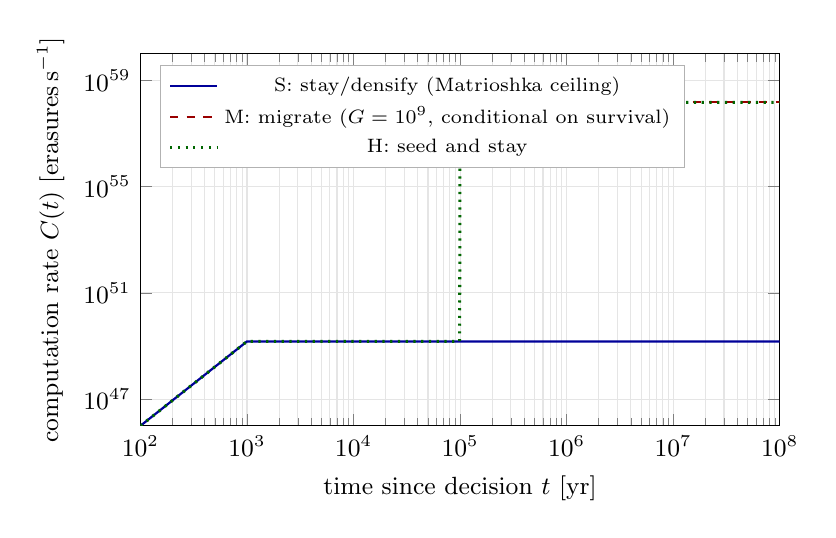
\begin{tikzpicture}
\begin{loglogaxis}[
  width=0.8\textwidth, height=0.52\textwidth,
  xlabel={time since decision $t$ [yr]},
  ylabel={computation rate $C(t)$ [erasures\,s$^{-1}$]},
  xmin=1e2, xmax=1e8, ymin=1e46, ymax=1e60,
  grid=both, grid style={black!10},
  tick label style={font=\small}, label style={font=\small},
  legend style={font=\scriptsize, at={(0.03,0.97)}, anchor=north west, draw=black!30}
]
% S: flat at 1.5e49 from t=1e3
\addplot[thick, blue!60!black] coordinates {(1e2,1e46) (1e3,1.5e49) (1e8,1.5e49)};
\addlegendentry{S: stay/densify (Matrioshka ceiling)}
% M: no output during transit; curve drawn only for t >= tau = 1e5
\addplot[thick, red!60!black, dashed] coordinates {(1e5,1.5e58) (1e8,1.5e58)};
\addlegendentry{M: migrate ($G = 10^{9}$, conditional on survival)}
% H: S then S+M
\addplot[thick, green!40!black, dotted, line width=1.1pt] coordinates {(1e2,1e46) (1e3,1.5e49) (9.9e4,1.5e49) (1e5,1.5e58) (1e8,1.5e58)};
\addlegendentry{H: seed and stay}
\end{loglogaxis}
\end{tikzpicture}
\caption{Undiscounted computation-rate histories for the three strategies at fiducial parameters (Table~\ref{tab:params}). Strategy S reaches its radiator-limited ceiling (Eq.~\ref{eq:cs}) within centuries and holds it. Strategy M delivers nothing for $\tau = 10^{5}$~yr (its curve is drawn only for $t \geq \tau$; during transit there is no output), then a rate $G = 10^{9}$ times higher, conditional on transit survival. The hybrid follows S until the seed's destination comes online, then collects both; strictly its early segment is $(1-f)\,C_{\mathrm S}$ plus the seed line, an offset invisible at this scale for $f \leq 10^{-6}$. The decision problem is whether the area under the M step, discounted and risk-weighted, exceeds the head start of S.}
\label{fig:kernels}
\end{figure}

% =====================================================================
\section{Crossover conditions}
\label{sec:crossover}

\subsection{Migrate versus stay}

From Eqs.~(\ref{eq:us})--(\ref{eq:um}), $U_{\mathrm M} > U_{\mathrm S}$ reduces to
\begin{equation}
\boxed{\;\rho + \lambda \;<\; \frac{\ln\!\big(G\,p_{s}\big)}{\tau}\;\equiv\;\rho^{*}.}
\label{eq:threshold}
\end{equation}
The threshold depends on the enormous multiplier only through its logarithm: the structural reason the result is robust to the order-of-magnitude uncertainties in $G$. At the fiducials ($G = 10^{9}$, $p_{s} = 0.5$, $\tau = 10^{5}$~yr),
\begin{equation}
\rho^{*} \;=\; \frac{\ln(5\times10^{8})}{10^{5}\ \mathrm{yr}} \;\simeq\; 2.0\times10^{-4}\ \mathrm{yr^{-1}},
\end{equation}
corresponding to a combined discount-plus-hazard half-life $t_{1/2} = \ln 2/\rho^{*} \approx 3{,}500$~yr; this is a planning half-life in the usual sense only under $\lambda = 0$, since the threshold binds the sum $\rho + \lambda$, not the discount rate alone. Any lineage whose effective concern horizon exceeds a few millennia (a modest demand against the $10^{8}$-yr coherence the family's architectures assume elsewhere) prefers migration to densification. Under the full efficiency stack ($G = 10^{21}$) the threshold rises to $\rho^{*} \approx 4.8\times10^{-4}$~yr$^{-1}$ ($t_{1/2} \approx 1{,}400$~yr); under a pessimistic $p_{s} = 0.01$ it falls only to $1.6\times10^{-4}$~yr$^{-1}$, and even $p_{s} = 10^{-4}$ moves it only to $1.15\times10^{-4}$~yr$^{-1}$, a factor of 1.7; transit risk is nearly irrelevant inside the logarithm and the operative lever is the transit time $\tau$.

Because $\rho^{*} \propto 1/\tau$ linearly, $\tau$ is the one parameter where a factor of a few moves the answer, and the deceleration allowance of Section~\ref{sec:parameters} acts on $\tau$ directly. Table~\ref{tab:tausens} propagates it: if braking multiplies the cruise time by 2--3, the threshold falls to $0.7$--$1.0\times10^{-4}$~yr$^{-1}$ and the headline half-life lengthens to $\sim$$7$--$10$~kyr. The qualitative conclusion (patience horizons of millennia, against the $10^{8}$-yr coherence assumed elsewhere in the family) is unchanged; the quoted $3{,}500$-yr figure is the no-braking end of the band.

\begin{table}[tbp]
\centering
\caption{Sensitivity of the patience threshold to the transit-plus-construction time $\tau$, at fixed $G p_{s} = 5\times10^{8}$. The $\tau = 10^{5}$~yr row is the fiducial (bare cruise); the larger values represent deceleration by magsail or drag multiplying the cruise time by 2--3 \citep{ZubrinAndrews1991,PerakisHein2016,HellerHippke2017}.}
\label{tab:tausens}
\small
\begin{tabular}{lcc}
\toprule
$\tau$ [yr] & $\rho^{*} = \ln(G p_{s})/\tau$ [yr$^{-1}$] & $t_{1/2} = \ln 2/\rho^{*}$ [yr] \\
\midrule
$1\times10^{5}$ & $2.0\times10^{-4}$ & $3{,}500$ \\
$2\times10^{5}$ & $1.0\times10^{-4}$ & $6{,}900$ \\
$3\times10^{5}$ & $6.7\times10^{-5}$ & $10{,}400$ \\
\bottomrule
\end{tabular}
\end{table}

The $p_{s} = 0.5$ fiducial is anchored, loosely, in the only quantitative literature on transit attrition: \citet{Hoang2017} model gas and dust damage to relativistic spacecraft and find survivable but non-negligible erosion at $0.2c$ over the parsec-scale column to $\alpha$~Centauri. Over kiloparsec columns the damage integral is $\sim$$4\times10^{3}$ times larger and mitigation (shielding, redundancy, en-route repair) is unmodelled, so 0.5 should be read as an order-unity placeholder rather than a conservative bound; the logarithmic dependence just exhibited is what makes this imprecision tolerable. Note that $p_{s}$ prices transit alone. Post-arrival residence survival inside the operating envelope is $\approx 0.8$ over $10^{8}$~yr at Paper E's fiducial remnant fraction: Paper E's flyby accounting with mass-segregated remnants now carries two curves. Its conservative impulsive floor is $\sim$$6\times10^{7}$~yr at $f_{\mathrm{BH}} = 0.01$ with the revised $31\,\msun$ perturber mass; its adiabatically corrected estimate, which is the physical one, has an envelope minimum of $3\times10^{8}$~yr and reaches the cluster-age cap in the interior. The $\approx 0.8$ figure is supported by the corrected curve with margin, and the impulsive floor is the conservative alternative. The dominant recurrent hazard, tidal-disruption-event loading with recurrence $\gtrsim 10^{7}$~yr, is survivable by engineered response and enters the deferred payoff only as a small amortization correction on that horizon \citep{Swanson2026Engineered}. The logarithmic entry of $p_{s}$ just exhibited is what keeps the threshold stable against that revision.

Figure~\ref{fig:crossover} maps $\rho^{*}$ against destination distance for the beamed-sail speed range, marking named Galactic targets. Because $\tau \propto d$, the threshold scales as $1/d$: closer acceptable destinations relax the patience requirement proportionally, which is one economic reading of Paper A's selection pressure toward the nearest adequate system rather than the best one. The $\omega$~Cen marker sits at $\rho^{*} = 2.24\times10^{-4}$~yr$^{-1}$, slightly above the fiducial $2.0\times10^{-4}$~yr$^{-1}$ quoted above, because the figure uses the bare transit time at $v = 0.2c$ ($\tau = d/v \approx 8.95\times10^{4}$~yr) while the fiducial rounds $\tau$ up to $10^{5}$~yr to include construction.

\begin{figure}[tbp]
\centering
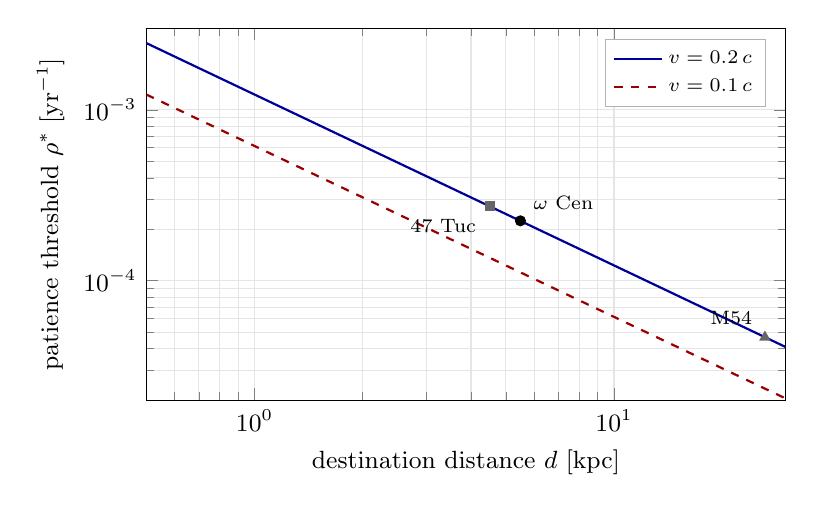
\begin{tikzpicture}
\begin{loglogaxis}[
  width=0.8\textwidth, height=0.52\textwidth,
  xlabel={destination distance $d$ [kpc]},
  ylabel={patience threshold $\rho^{*}$ [yr$^{-1}$]},
  xmin=0.5, xmax=30, ymin=2e-5, ymax=3e-3,
  grid=both, grid style={black!10},
  tick label style={font=\small}, label style={font=\small},
  legend style={font=\scriptsize, at={(0.97,0.97)}, anchor=north east, draw=black!30}
]
% rho* = ln(5e8) / (d[kpc]*3261.6/v[c] yr) ; v=0.2: tau= d*16308 yr; v=0.1: tau = d*32616
\addplot[thick, blue!60!black, domain=0.5:30, samples=40] {20.03/(x*16308)};
\addlegendentry{$v = 0.2\,c$}
\addplot[thick, red!60!black, dashed, domain=0.5:30, samples=40] {20.03/(x*32616)};
\addlegendentry{$v = 0.1\,c$}
% omega Cen at 5.49 kpc
\addplot[only marks, mark=*, mark size=1.8pt, black] coordinates {(5.49,2.24e-4)};
\node[font=\scriptsize, anchor=south west] at (axis cs:5.6,2.3e-4) {$\omega$ Cen};
\addplot[only marks, mark=square*, mark size=1.6pt, black!60] coordinates {(4.52,2.72e-4)};
\node[font=\scriptsize, anchor=north east] at (axis cs:4.4,2.6e-4) {47 Tuc};
\addplot[only marks, mark=triangle*, mark size=2.0pt, black!60] coordinates {(26.28,4.67e-5)};
\node[font=\scriptsize, anchor=south east] at (axis cs:25.8,4.85e-5) {M54};
\end{loglogaxis}
\end{tikzpicture}
\caption{The patience threshold $\rho^{*} = \ln(G p_{s})/\tau$ (Eq.~\ref{eq:threshold}) versus destination distance, for the beamed-sail speed range and fiducial $G p_{s} = 5\times10^{8}$. A lineage migrates when its combined discount-plus-hazard rate falls below the curve. Named points assume the marker's cluster is the nearest adequate destination for the deciding lineage; distances from \citet{BaumgardtVasiliev2021}. The logarithmic dependence on $G p_{s}$ means order-of-magnitude changes in the multiplier or the risk shift these curves by less than a factor of 2.5. Both curves use the bare cruise time $\tau = d/v$; deceleration multiplying $\tau$ by 2--3 lowers them by the same factor (Table~\ref{tab:tausens}).}
\label{fig:crossover}
\end{figure}

\subsection{What the threshold means}

Equation~(\ref{eq:threshold}) converts the inward-family debate into a single empirical-psychological question: do long-lived technological lineages discount the far future at more or less than a few parts in $10^{4}$ per year? The literature's positions map onto the two sides. \citet{Bostrom2003} argues that agents with astronomical stakes should approach $\rho = 0$; on his side of the line, migration dominates by many orders of magnitude. Steep discounters (lineages whose institutions cannot sustain plans beyond centuries) stay home and densify, and for them the inward family predicts nothing. The threshold also prices the goal-stability problem: Eq.~(\ref{eq:threshold}) says the plan need only survive attrition at the few-per-$10^{4}$ annual rate during the transit window, not for the $10^{8}$-yr exploitation phases that follow (see Eq.~\ref{eq:umus}), and post-arrival value drift merely redistributes the payoff among successor agents while leaving the dynamical residues of Paper A in place. Under the symmetric valuation of Section~\ref{sec:kernels} this transit-window reading holds whether $\lambda$ prices lineage death or plan abandonment; the residual asymmetry is that a deliberating lineage in transit is exposed to institutional-drift channels a non-deliberating payload is not, one more consideration favouring seeds over whole-lineage relocation.

% =====================================================================
\section{The hybrid result}
\label{sec:hybrid}

\subsection{Dominance}

Comparing Eq.~(\ref{eq:uh}) with Eqs.~(\ref{eq:us}) and (\ref{eq:um}): under additive utility and a full-fidelity seed, $U_{\mathrm H} > U_{\mathrm M}$ in one line (the stay component is pure addition), and $U_{\mathrm H} > U_{\mathrm S}$ whenever
\begin{equation}
f \;<\; G\, p_{s}\, e^{-(\rho+\lambda)\tau}.
\label{eq:hybrid}
\end{equation}
The right-hand side at fiducials is $\sim$$5\times10^{8}\,e^{-20\,(\rho+\lambda)/\rho^{*}}$, and the exponential is unforgiving: at the migration threshold itself the tolerable seed cost is $5\times10^{8}e^{-20} \sim 1$, but at $\rho + \lambda = 2\rho^{*}$ it has fallen to $\sim$$2\times10^{-9}$, and at $10\rho^{*}$ to $\sim$$10^{-78}$. The physical seed cost, gram-to-kilogram payloads plus a launch array \citep{Lubin2016,Freitas1980}, is tiny against a Dyson-scale economy: \citet{Armstrong2013} estimate that seeding every galaxy within several hundred Mpc costs a small fraction of one star's output, which supports $f \lesssim 10^{-6}$ a fortiori for a single Galactic destination. Setting $f = 10^{-6}$ in Eq.~(\ref{eq:hybrid}) gives breakeven at $(\rho+\lambda)\tau = \ln(5\times10^{14}) \approx 34$, i.e.\ $\rho + \lambda \approx 1.7\,\rho^{*}$. The hybrid therefore dominates both pure strategies in a band extending modestly beyond the migration threshold, roughly $1.7\times$ the threshold at $f = 10^{-6}$ (and only logarithmically further for still-cheaper seeds), because the exponential discount on the deferred payoff crushes the seed's expected value within a factor of a few of $\rho^{*}$. Outside that band the utility calculus reverts to pure S; inside it, and everywhere migration itself clears, H is strictly best barring non-additive utilities (Section~\ref{sec:limits}).

The comparison with M is one line only under full seed fidelity. With the drift-weighted valuation of Section~\ref{sec:kernels}, $U_{\mathrm H} = (1-f)\,U_{\mathrm S} + p_{d}\,U_{\mathrm M}$, and H beats M only if $(1-f)\,U_{\mathrm S} > (1-p_{d})\,U_{\mathrm M}$; deep in migration-favourable territory ($U_{\mathrm M}/U_{\mathrm S} \approx 2.3\times10^{4}$ at $\rho+\lambda = 0.5\,\rho^{*}$) that requires $1 - p_{d} \lesssim 4\times10^{-5}$ if M itself is credited at full fidelity. The rescuing assumption, stated here because the dominance claim rests on it: a migrating lineage carries its own drift factor $p_{d}^{\mathrm M}$ over the same horizon, and a non-deliberating seed drifts no more than a deliberating lineage in transit ($p_{d} \geq p_{d}^{\mathrm M}$), whence $U_{\mathrm H} \geq U_{\mathrm M}$ term by term. Given that assumption, the dominance itself is close to a bookkeeping identity; the substantive content of this section is the narrowness of the band beyond the threshold, $1.7\,\rho^{*}$ at $f = 10^{-6}$, given a nearly free seed.

\subsection{Consequences}

The dominance of H restructures the Fermi implications of the family in three ways.

First, compliance is cheap for the patient. The incomplete-compliance objection (Paper B, problem P4) imagines lineages weighing a costly relocation and many declining. Under H there is no relocation to decline: dispatching seeds is compatible with staying, and the marginal cost is negligible against Dyson-scale output. For every lineage inside the dominance band ($\rho+\lambda \lesssim 1.7\,\rho^{*}$), the question ``what fraction migrates?'' becomes ``what fraction of computation-valuing lineages fails to spend $f \sim 10^{-6}$ of output on a large expected return?'' The compliance question is thereby displaced, not dissolved: it becomes the question of what fraction of maximizers sit below the modestly enlarged threshold, which is a claim about the distribution of $\rho + \lambda$ rather than about willingness to pay.

Second, destinations saturate early. If seeds are cheap, the nearest adequate IMBH systems receive seeds from every computation-valuing lineage in their neighbourhood, and first arrival plausibly matters. This turns the uncontested-claim criterion of Paper A (criterion 3) into a race dynamic of the kind \citet{Hanson1998} analysed for interstellar colonization generally, in which selection favours the fastest and least encumbered colonizers of contested oases, and it implies that the residues of Paper A's P4 should be present in suitable systems even if no lineage ever ``migrates'' in the whole-population sense. One scope note: the threshold of Eq.~(\ref{eq:threshold}) is a single-agent calculation, and competition for contested oases only lowers it, since preemption adds option value to early arrival; Eq.~(\ref{eq:threshold}) is therefore an upper bound on the patience required.

The apparent conflict with Paper A's uncontested-claim criterion resolves by economic era rather than by contradiction: the destination is uncontested by fusion-era economics, for which low-mass cluster stars are poor assets, and maximally contested among computation-maximizing lineages, for which they are the prize; this is the form in which Paper A now states criterion 3, and it is the resolution both papers adopt. Congestion also enters the threshold only logarithmically. If $k$ lineages arrive and share the destination, the per-lineage gain is $G/k$ and the threshold shifts by $\ln k$ inside Eq.~(\ref{eq:threshold}); if the destination is winner-take-all, the survival factor becomes $p_{s}/k$, with the same logarithmic entry. For $k \lesssim 10^{2}$ the shift is smaller than the uncertainties already carried in $G$, so the single-agent threshold stands.

Third, the loud residue does not vanish. Under pure M, migrated lineages leave planetary space entirely and the sky is silent. Under dominant H, the stay component continues local densification, whose Matrioshka waste heat is the classic detectable technosignature \citep{Dyson1960,Wright2014}. The hybrid therefore predicts both residue classes in linked proportion, the basis of the new population statistic in Section~\ref{sec:residues}.

% =====================================================================
\section{Population consequences}
\label{sec:population}

Let a fraction $x$ of long-lived technological lineages be expansionists, the class supplying the loud signals whose absence constitutes the paradox \citep{Hanson2021,Olson2015}; the remainder are satisficers and other quiet types that contribute nothing to $N_{\rm loud}$ regardless of the inward gradient. Expansionism and computation maximization are not exclusive: a lineage can expand and also value integrated computation, and it is that overlap the inward family acts on. Within the expansionist class, let $q$ be the fraction susceptible to the inward gradient, that is, the conditional probability that an expansionist also holds the P1 optimization goal, so that the gradient bears on its behaviour at all. Within that susceptible subset, let $m$ be the fraction whose parameters fall below the (hybrid-enlarged) threshold of Section~\ref{sec:hybrid}, and $w \in [0,1]$ the capture weight: the probability that susceptibility plus a cleared threshold actually converts loud expansion into quiet inward behaviour before or during the expansion phase.

The inward family's contribution to the silence is the claim, argued qualitatively in Paper A, that the maximizer subset contains the oldest and most capable lineages, so its withdrawal from loud behaviour thins the expected loud population disproportionately. The expected number of loud civilizations in a survey volume containing $N$ lineages is
\begin{equation}
N_{\rm loud} \;=\; N\big[\,x\,(1 - w\,q\,m)\,\big],
\label{eq:thinning}
\end{equation}
with $q$, $m$, and $w$ the nested conditional fractions defined above, so that $w q m$ is the capture probability for a randomly drawn expansionist. Equation~(\ref{eq:thinning}) identifies only the product $wqm$: a measured $N_{\rm loud}$ constrains one number, and the $(q,w)$ grid below is a re-parameterization of that single degree of freedom, useful for exhibiting which value combinations reach it, not evidence of two independently constrained parameters.

One step separates $N_{\rm loud}$ from anything observed, and it is not small. $N_{\rm loud}$ counts loud civilizations that \emph{exist}; the surveys invoked in Section~\ref{sec:residues} bound the number that would have been \emph{detected}, so the silence condition is $N_{\rm loud}\,\langle p_{\rm det}\rangle < 1$, with $\langle p_{\rm det}\rangle$ the completeness of those surveys for the signature in question. For Galactic Matrioshka-class sources that completeness is well below unity and is distance- and temperature-limited in the ways Section~\ref{sec:residues} describes \citep{Carrigan2009,Zackrisson2018}. Table~\ref{tab:thinning} is therefore evaluated at $\langle p_{\rm det}\rangle = 1$ and its bold cells are the most restrictive corner of the condition; any realistic completeness widens the silence-compatible region, in some cases substantially. We tabulate the $\langle p_{\rm det}\rangle = 1$ case because it is the one that does not require a survey-completeness model this paper has no means to supply, and we flag the direction of the bias rather than absorb it. For the potential-expansionist count $N x$, the dissolution analysis of \citet{SandbergDrexlerOrd2018} shows that reasonable uncertainty over the Drake factors puts substantial probability on $N x$ of order unity as well as on large values, which is why we tabulate three decades of it. The three rows are scenarios, not equally weighted hypotheses: that analysis produces a posterior on $N$ given the silence, and it places its largest mass on the low branch, where no inward capture is needed to dissolve the paradox at all. We tabulate the high branches because the family's contribution is only interesting there, not because they carry equal weight. Table~\ref{tab:thinning} evaluates the silence-compatibility condition $N_{\rm loud} < 1$ across the $(q, w)$ grid for three values of the potential-expansionist count $N x$. The table's message matches what Papers A and B anticipated, with the dependence on $N x$ making the thinning claim quantitative rather than binary. At the fiducial $N x = 10$, inward capture alone dissolves the paradox only in the complete-capture corner ($w q \to 1$); at moderate capture it thins the expectation by factors of a few and the balance must come from conventional rarity. At $N x = 100$ even complete capture of the maximizer subset leaves the paradox intact unless $q \to 1$, so the family there functions only as a rarity multiplier. At $N x = 3$ the silence condition opens up: capture products $w q \gtrsim 0.7$ suffice, and several non-degenerate cells satisfy $N_{\rm loud} < 1$ without full compliance. Hybrid dominance no longer drives $m \to 1$ across the board: Section~\ref{sec:hybrid} enlarges the acting region only to $\rho+\lambda \lesssim 1.7\,\rho^{*}$, so $m$ is the fraction of susceptible expansionists below that modestly enlarged threshold and remains a live economic parameter alongside $q$ and $w$. The residual uncertainty therefore splits between the distribution of patience ($m$) and the distribution of terminal values ($q$, $w$), with the economics of this paper constraining only the first.

\begin{table}[tbp]
\centering
\caption{Expected loud count $N_{\rm loud}$ (Eq.~\ref{eq:thinning}) for three values of the potential-expansionist count $N x$ per survey volume ($N x = 10$ fiducial), with $q$ the fraction of expansionists susceptible to the inward gradient, $w$ the capture weight, and $m = 1$ throughout (entries are lower bounds on $N_{\rm loud}$ when part of the population discounts above $\sim$$1.7\,\rho^{*}$). Silence requires $N_{\rm loud} < 1$ (bold). Only the single product $wqm$ enters Eq.~(\ref{eq:thinning}); the grid re-parameterizes that one degree of freedom to exhibit which combinations reach silence.}
\label{tab:thinning}
\small
\begin{tabular}{llcccc}
\toprule
 & & $w = 0.25$ & $w = 0.5$ & $w = 0.75$ & $w = 1$ \\
\midrule
$N x = 3$
 & $q = 0.25$ & 2.8 & 2.6 & 2.4 & 2.3 \\
 & $q = 0.5$  & 2.6 & 2.3 & 1.9 & 1.5 \\
 & $q = 0.75$ & 2.4 & 1.9 & 1.3 & \textbf{0.8} \\
 & $q = 1$    & 2.3 & 1.5 & \textbf{0.8} & \textbf{0.0} \\
\midrule
$N x = 10$
 & $q = 0.25$ & 9.4 & 8.8 & 8.1 & 7.5 \\
 & $q = 0.5$  & 8.8 & 7.5 & 6.3 & 5.0 \\
 & $q = 0.75$ & 8.1 & 6.3 & 4.4 & 2.5 \\
 & $q = 1$    & 7.5 & 5.0 & 2.5 & \textbf{0.0} \\
\midrule
$N x = 100$
 & $q = 0.25$ & 94 & 88 & 81 & 75 \\
 & $q = 0.5$  & 88 & 75 & 63 & 50 \\
 & $q = 0.75$ & 81 & 63 & 44 & 25 \\
 & $q = 1$    & 75 & 50 & 25 & \textbf{0.0} \\
\bottomrule
\end{tabular}
\end{table}

% =====================================================================
\section{Observational corollaries: the residue ratio}
\label{sec:residues}

\specbox{This section converts the decision analysis into population-level observables. It inherits all conditionality of the optimization premise.}

Hybrid dominance predicts linked residues: for every lineage acting on the gradient, a continuing local densification (Matrioshka-class mid-infrared source) and a seeded quiet-cluster system (the Paper A dynamical residues: anomalous spin, suppressed accretion, core depletion). Pure M predicts quiet clusters without Matrioshka sources; pure S the reverse. The observable is the sky ratio
\begin{equation}
R_{\rm sky} \;\equiv\; \frac{N_{\rm Matrioshka}}{N_{\rm quiet\mathchar`-cluster\ residue}} \;=\;
\begin{cases}
\;0 & \text{pure M} \\[2pt]
\;\mathcal{O}(1)\times\dfrac{n_{\rm lineage}}{n_{\rm target}} & \text{hybrid H} \\[4pt]
\;\infty & \text{pure S,}
\end{cases}
\label{eq:ratio}
\end{equation}
where $n_{\rm lineage}/n_{\rm target}$ is the ratio of acting lineages to adequate destination systems in the relevant volume (several lineages can seed one cluster; one lineage densifies one home system). The Milky Way contains $\sim$$150$ globular clusters of which a handful satisfy the Paper A criteria, so under H with even a few Galactic lineages the formation-rate ratio satisfies $R \gtrsim 1$.

The observed ratio is a snapshot, however, and the two residue classes have very different lifetimes. Paper E's cascade analysis finds that an abandoned Matrioshka-class swarm collides itself into debris on $10^{2}$--$10^{3}$~yr and (at the destination) drains into the hole, so dead installations vanish quickly and only actively maintained ones radiate; the quiet-cluster dynamical residues (anomalous spin above all, the one fossil that outlasts the Hubble time) persist for $\gtrsim$~Gyr \citep{Swanson2026Engineered}. The observable sky ratio is therefore the formation-rate ratio multiplied by a lifetime ratio, $R_{\rm obs} = R \times (t_{\rm Matrioshka}/t_{\rm residue})$, and if home installations are maintained only while the lineage remains interested, $t_{\rm Matrioshka}/t_{\rm residue}$ can be $\ll 1$, driving $R_{\rm obs} \ll 1$ even under fully compliant H.

This puts existing null results to work, with the lifetime factor carried explicitly. For extragalactic waste heat, the WISE-based $\hat{G}$ surveys \citep{Wright2014,Griffith2015} bound galaxy-scale reprocessed emission in $\sim$$10^{5}$ external galaxies; for Galactic Dyson- and Matrioshka-class sources, the operative bounds are the IRAS search of \citet{Carrigan2009}, the Gaia/2MASS-selected candidate analysis of \citet{Zackrisson2018}, and the Project Hephaistos series: \citet{Suazo2024} report seven unresolved Galactic candidates surviving their photometric cuts, most or all of which subsequent analyses attribute to hot-dust-obscured background AGN contamination \citep{Ren2024,Blain2024,Ren2025}. Together these bound $N_{\rm Matrioshka}$ in the Galaxy at or near zero over their completeness ranges, pending contamination analysis of the surviving Hephaistos candidates. Through Eq.~(\ref{eq:ratio}), those bounds propagate to the hybrid branch only after division by the lifetime ratio, and the propagation is a limit rather than a deduction. With $N_{\rm Matrioshka}$ observed as zero, the ratio $N_{\rm Matrioshka}/N_{\rm quiet}$ carries no information about its own denominator; what the data support is a joint Poisson likelihood on the two counts with $R_{\rm obs}$ as a parameter, from which an upper limit on $N_{\rm quiet}$ follows only through an assumed $R_{\rm obs}$ and its uncertainty. Stated that way: if $R_{\rm sky,obs} \gtrsim 1$ (long-maintained home installations), the infrared nulls place a comparable upper limit on $N_{\rm quiet\mathchar`-cluster\ residue}$, and the family's Galactic prediction concentrates on the pure-M corner: lineages whose utilities are non-additive across descendants (Section~\ref{sec:limits}) or whose home infrastructure is dismantled at departure. If instead maintenance lifetimes are short, the infrared nulls carry little weight against H and the quiet-cluster channel is left unconstrained by them. The Paper C campaign tests the quiet-cluster channel directly at $\omega$~Cen either way. Conversely, a confirmed Paper A residue (a near-extremal spin on a gas-starved IMBH) with a continuing Matrioshka null would be evidence about the utility structure of whatever laid the residue down: it would indicate migration without a maintained home presence, the signature of either whole-lineage relocation or post-departure home abandonment. That a spin measurement could carry information about value structure is an inference this pricing framework licenses; we state it in advance of any data.

The archival anomaly-detection agenda of the Dyson Minds workshop \citep{Curtis2026DysonMinds} and the cluster-ranking metrics of \citet{Huang2026Crystallization} both operate on the two source classes Eq.~(\ref{eq:ratio}) links; a joint analysis (ranking clusters and IR-anomaly candidates in the same volume and testing the correlation Eq.~(\ref{eq:ratio}) implies) is executable from public archives and is, to our knowledge, unproposed.

% =====================================================================
\section{Limits and objections}
\label{sec:limits}

\paragraph{Model dependence of the utility.} Equation~(\ref{eq:utility}) assumes utility linear in computation rate and additive across locations and descendants. Identity-centred utilities break additivity: a lineage that values only its own continuous thread of computation may not credit a forked seed's output, restoring the pure S-versus-M choice of Section~\ref{sec:crossover}, which is why the crossover analysis is retained rather than replaced by the hybrid result. Satisficing utilities (compute enough, not most) exit the framework entirely; they belong to the sustainability solution \citep{HaqqMisraBaum2009}, not to the inward family.

\paragraph{Discounting form.} Exponential discounting is the tractable choice, and no directional claim survives its relaxation cleanly. Hyperbolic discounters \citep{Laibson1997} have low long-run rates, but they are time-inconsistent: the deciding present self applies its steep short-run rate to the whole deferred payoff at the moment of choice, so hyperbolic discounting does not automatically favour migration. The outcome depends on sophistication: a naive hyperbolic agent perpetually postpones a launch it always ``intends'' to make, while a sophisticated one may commit early (a seed, once launched, is a commitment device immune to later preference reversals, one more argument for H over M). A genuinely zero-discount agent \citep{Ramsey1928,Bostrom2003} is handled by the finite-horizon kernel of Section~\ref{sec:kernels}: the infinite-horizon utilities diverge at $\rho + \lambda = 0$, but the ratio of Eq.~(\ref{eq:finitehorizon}) remains defined and migration wins by the capped factor $p_{s} G\, T_{\mathrm M}/T_{\mathrm S} \approx 5\times10^{4}$--$5\times10^{6}$.

Uncertainty about the discount rate pushes the same direction, and more forcefully. Under gamma (declining) discounting \citep{Weitzman1998,Weitzman2001}, an agent uncertain over its own $\rho$ values the far future by the expectation of the discount factor, giving a certainty-equivalent rate
\begin{equation}
\rho_{\rm eff}(t) \;=\; -\frac{1}{t}\,\ln \mathbb{E}\!\left[e^{-\rho t}\right],
\label{eq:gamma}
\end{equation}
which declines with horizon toward the minimum plausible rate: the patient scenarios dominate the expectation at long $t$. An agent placing equal weight on $\rho = 10^{-3}$ and $\rho = 10^{-6}$ has $\rho_{\rm eff}(\tau) = -\ln[\tfrac12(e^{-100} + e^{-0.1})]/\tau \approx 7.9\times10^{-6}$~yr$^{-1}$ at $\tau = 10^{5}$~yr (the certainty-equivalent rate approaches the $10^{-6}$ floor only at $t \gtrsim 10^{7}$~yr), still a factor of 25 below the threshold of Eq.~(\ref{eq:threshold}). Migration therefore requires only uncertainty about patience, not patience itself, which strengthens the case beyond the exponential baseline. For calibration in the other direction, empirical institutional discount rates are $10^{-2}$--$10^{-3}$~yr$^{-1}$, failing the threshold by up to two orders of magnitude: the framework describes old lineages, not present-day institutions.

\paragraph{Why not wait for faster sails?} \citet{Heller2017} showed that a civilization expecting propulsion to improve faces an incentive trap: launching now can be dominated by waiting for a faster vehicle that overtakes the earlier one. In this framework the trap does not bind. Waiting costs discounted utility at the rate $\rho + \lambda$ on the entire deferred payoff, while speed improvements enter only through $\tau \propto 1/v$ inside the same energy economics that already caps beamed sails at $0.1$--$0.2c$; a bounded reduction in $\tau$ cannot repay an open-ended delay, and the seed option makes the launch cost too small for the saving to matter.

\paragraph{Real options.} The migration decision is the canonical problem of irreversible investment under uncertainty \citep{McDonaldSiegel1986,DixitPindyck1994}, and the wait-for-sails argument above is an informal option-value comparison. In the deterministic setup of this paper the option to defer is worthless: with $v$, $G$, and $\tau$ known, waiting buys no information, only discounting, which is the conclusion of the preceding paragraph restated in that literature's terms. The seed strategy then has a standard name: it buys the option cheaply rather than exercising it, holding the deferred claim at cost $f$ while the state of the world reveals itself. A full treatment requires stochastic dynamics for $v$ or $G$ (a Poisson-arrival improvement process is the natural minimal model) and is deferred.

\paragraph{The hazard rate is not a solution to goal stability.} Folding P2 into $\lambda$ prices the problem; it does not solve it. What the pricing shows is the problem's true size: under either reading of $\lambda$ given the symmetric valuation of Section~\ref{sec:kernels}, coherence is required at the few-per-$10^{4}$-per-year level during transit only (Section~\ref{sec:crossover}), a far weaker demand than the $10^{8}$-yr coherence the exploitation architecture assumes, and one that seed automation (a payload that does not deliberate en route) plausibly meets by construction; the residual seed-side drift is carried continuously by the valuation factor $p_{d}$ of Section~\ref{sec:kernels} rather than as an all-or-nothing loss. The deep version of P2 (whether the destination civilization retains the values that sent it) remains open and remains, as Paper B noted, not an astronomy problem.

\paragraph{Parameter unmeasurability.} $q$, $w$, $\rho$, $\lambda$ are distributions over agents we have never observed. The defensible claims are structural: the logarithmic insensitivity of the threshold (Eq.~\ref{eq:threshold}), the dominance region of the hybrid (Eq.~\ref{eq:hybrid}), and the sign of the residue-ratio prediction (Eq.~\ref{eq:ratio}). Point estimates in this paper are fiducials for orientation, not forecasts.

\paragraph{Grabby-aliens integration.} The \citet{Hanson2021} machinery conditions on our early arrival to bound the density of loud expanders. Equation~(\ref{eq:thinning}) plugs into that frame by modifying the loud fraction while leaving the arrival-time statistics unchanged: inward capture reduces the volume-conversion rate of loud lineages without changing when civilizations arise. A full integration (re-deriving the grabby-aliens posterior with a capture term) is beyond this paper's scope and is the natural next step for whoever takes up Paper B's problem P1; Eq.~(\ref{eq:thinning}) supplies the term to insert.

\paragraph{Outward counter-positions.} \citet{Ivliev2026} (preprint, submitted to \emph{Acta Astronautica}) argues from a comparable automation premise to the opposite directional conclusion: once autonomous AI industry crosses a capability threshold, quiet outward expansion through low-mass probes and seed factories becomes too cheap for any civilization to refuse, and the silence reflects expansion signatures too weak to detect rather than migration. The two frameworks agree that seeds are nearly free (his threshold argument and our Eq.~\ref{eq:hybrid} are the same observation) and disagree about the objective: under our kernels the same cheap automation buys more computation per unit resource by seeding inward than by saturating stellar systems, so the disagreement reduces to whether coverage or computation is the maximand, i.e.\ to the distribution of terminal values already carried by $q$ in Section~\ref{sec:population}.

Two further outward positions deserve engagement. \citet{Hooper2018} argues that a civilization anticipating accelerating cosmic expansion should harvest stars from surrounding volumes and bring them home before the horizon removes them, the strongest quantitative argument for outward action in the literature. The mechanism concedes this paper's core premise, mass relocation across kiloparsec scales in the service of future computation, and disputes only the direction; and its clock is the dark-energy horizon at $\sim$$10^{9}$--$10^{10}$~yr, which never binds the $\tau = 10^{5}$~yr decision analysed here: a lineage can seed inward now and harvest outward later without conflict between the two programmes. \citet{Ord2021} maps the affectable universe and reaches a structurally similar conclusion, that the resources within outward reach are bounded and shrinking, which if anything sharpens the case for optimizing what a lineage can already touch.

\paragraph{Anthropic caveats.} As with Paper A, our own existence as a young loud lineage neither confirms nor embarrasses the analysis; the framework describes the asymptotic behaviour of old lineages, and we are not one. Self-indication corrections to the population frame of Section~\ref{sec:population} are absorbed into the grabby-aliens integration deferred above.

% =====================================================================
\section{Conclusion}
\label{sec:conclusion}

Paper B posed the question this paper answers: under what conditions does relocation to a thermodynamically privileged destination beat staying home and building? The answer has three parts. The crossover between migration and densification is a patience threshold, $\rho + \lambda < \ln(G p_{s})/\tau$, whose logarithmic form makes it robust to the large uncertainties in the destination multiplier and transit risk; at fiducial parameters it asks only for combined discount-plus-hazard half-lives beyond a few thousand years. The seed-and-stay hybrid dominates both pure strategies throughout the migration-favourable region and in a band extending modestly beyond it, to roughly $1.7\times$ the threshold at physical seed costs, because the exponential discount on the deferred payoff closes the window quickly; within that band the incomplete-compliance problem reduces to the joint distribution of patience and the optimization goal. And the hybrid's linked residues yield a population-level prediction, a formation-rate ratio of Matrioshka sources to engineered clusters of order unity, which existing infrared nulls constrain only after weighting by the maintenance lifetime of home installations, concentrating the family's surviving parameter space on the pure-migration and short-maintenance corners that the $\omega$~Cen campaign of Paper C tests directly.

The broader point is methodological. The inward family has argued from thermodynamic gradients (Paper A), been organized and graded as a literature (Paper B), and acquired a costed observational program (Paper C). What it lacked was a demonstration that the gradient is economically actionable by agents with finite patience and fallible institutions, the step where favourable gradients often fail. This paper supplies that demonstration in closed form, with its assumptions priced and its observational consequences stated in advance. Whether any agent has ever faced the decision is a question for the instruments.

% =====================================================================
\section*{Acknowledgements and disclosure}

The author thanks the maintainers of the NASA Astrophysics Data System and arXiv, on which the citation verification for this work relied. The author's conflict of interest as proponent of the hypothesis whose economics this paper analyses is noted; the mitigation is the same as in the companion papers: closed-form results, conservative fiducials, and pre-stated observational consequences. \textbf{AI assistance disclosure:} drafting, citation verification, derivation checking, and figure preparation for this manuscript were performed with substantial assistance from a large language model (Claude, Anthropic), under the author's direction; the author reviewed and takes full responsibility for all claims, derivations, and references. Interactive calculators implementing the quantitative material in Sections~\ref{sec:kernels}--\ref{sec:residues} are available at \url{https://omegacentauri.me}.

\section*{Data availability}

No new observational data were generated for this work. All quantitative inputs derive from the cited literature.

\bibliographystyle{apalike}
\bibliography{references,campaign-extra,inward-extra,economics-extra}

\end{document}
